Figure \ref{fig:unloading-station-main} shows the elementary components of this station.
\FloatBarrier
\begin{figure}[h]
    \centering
    \includegraphics[width=0.95\textwidth]{figures/unloading-station.png}
    \caption{\parbox[t]{12cm}{Unloading station configuration. 1) Marker 2) Gantry 3) Magnetic gripper 4) Gripper 5) Inspection Camera 6) Control cabinets 7) KR1410 Teach pendant holder
    8) SIMATIC HMI}}
    \label{fig:unloading-station-main}
\end{figure}

\begin{enumerate}
    \item A marker is attached to the unloading station through which robot get the exact position of the unloading station.

    \item Similar to the storage station, the raw sheets are stored on a pull-out drawer. This also consists
    of a universal basic construction and an individual perforated grid plate. Depending on the type of
    sheet metal part, the blanks can be stacked on this perforated grid plate. The sheet metal parts can be
    held in place by means of sheet metal brackets that are screwed to the plate. Telescopic rails are also
    used here. Because the drawer does not have to be opened by a robot, but only by a person, rails with
    integrated locking mechanisms are used. Pulling out the drawer ensures ergonomically simple
    filling. The drawer position is monitored using a position switch. A gantry robot with a working area of $400 \times 1000 \times 250 mm$ is to be used for destacking.
    
    % \begin{figure}[h]
    %     \centering
    %     \begin{subfigure}{0.5\textwidth}
    %         \centering
    %         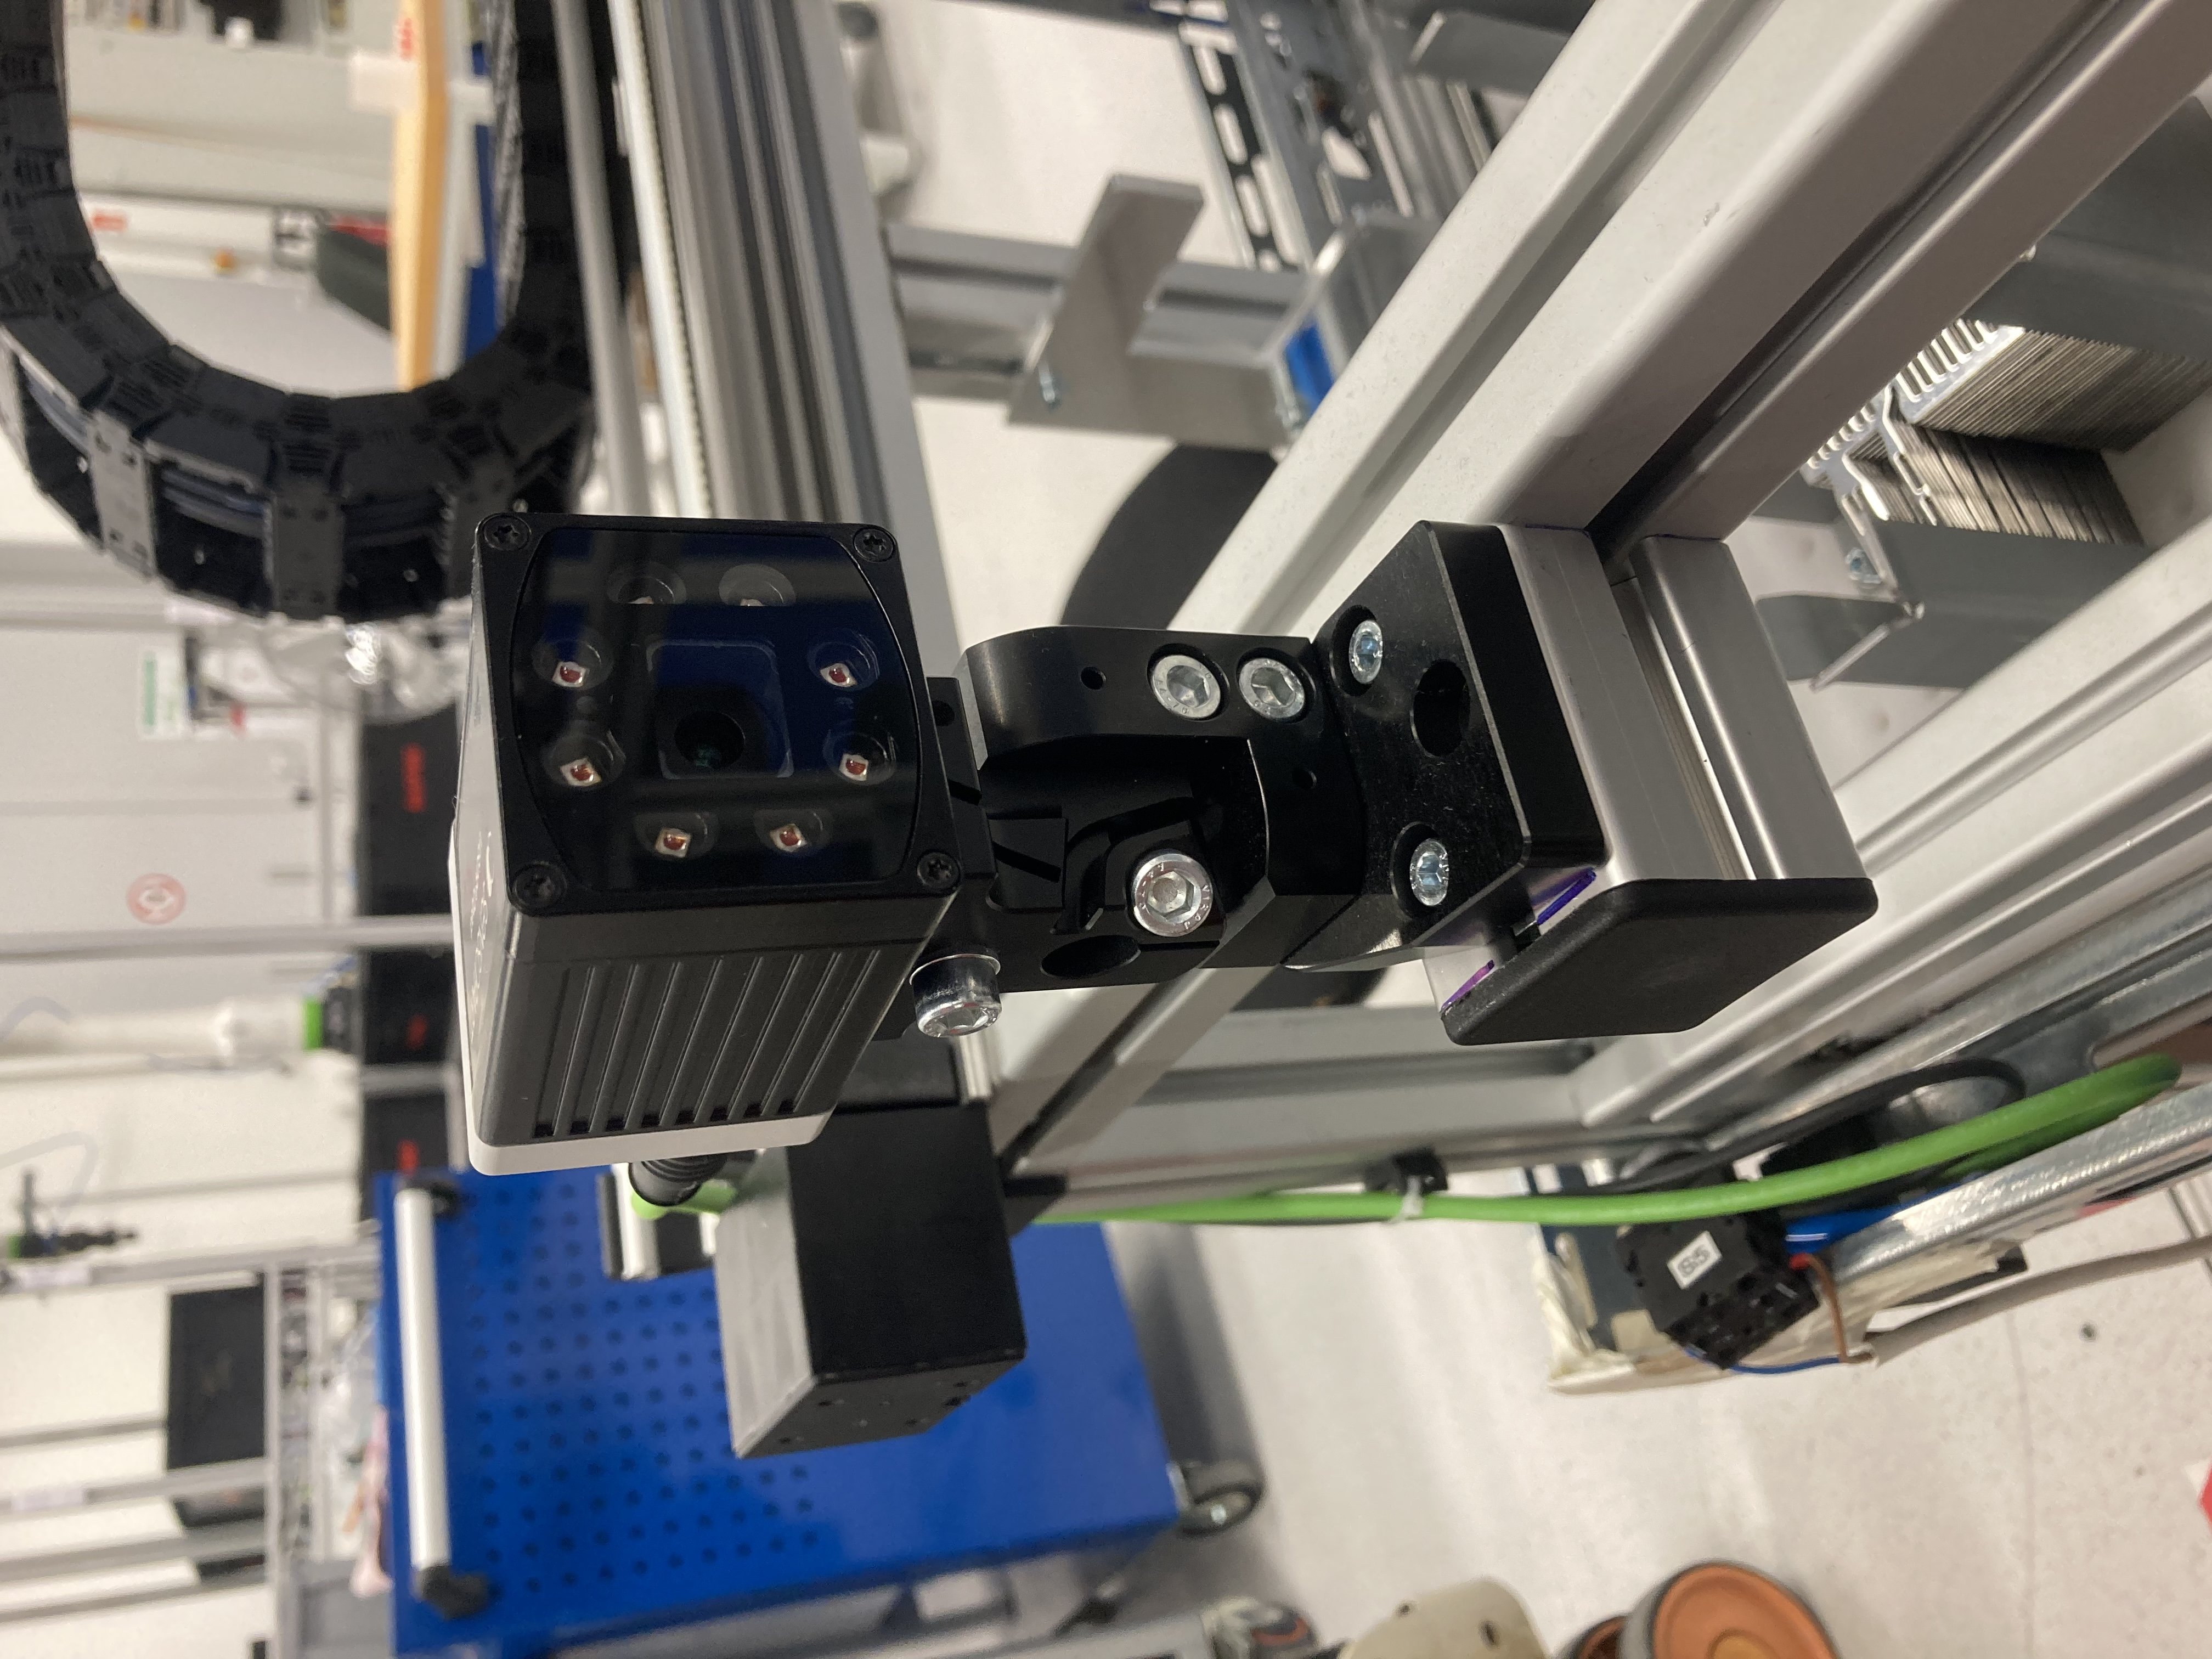
\includegraphics[width=\textwidth, angle=-90]{figures/inspection-camera.jpg} % Replace with your image file
    %         \caption{}
    %         \label{fig:inspection-camera}
    %     \end{subfigure}\hspace{-1.5cm}
    %     \begin{subfigure}{0.5\textwidth}
    %         \centering
    %         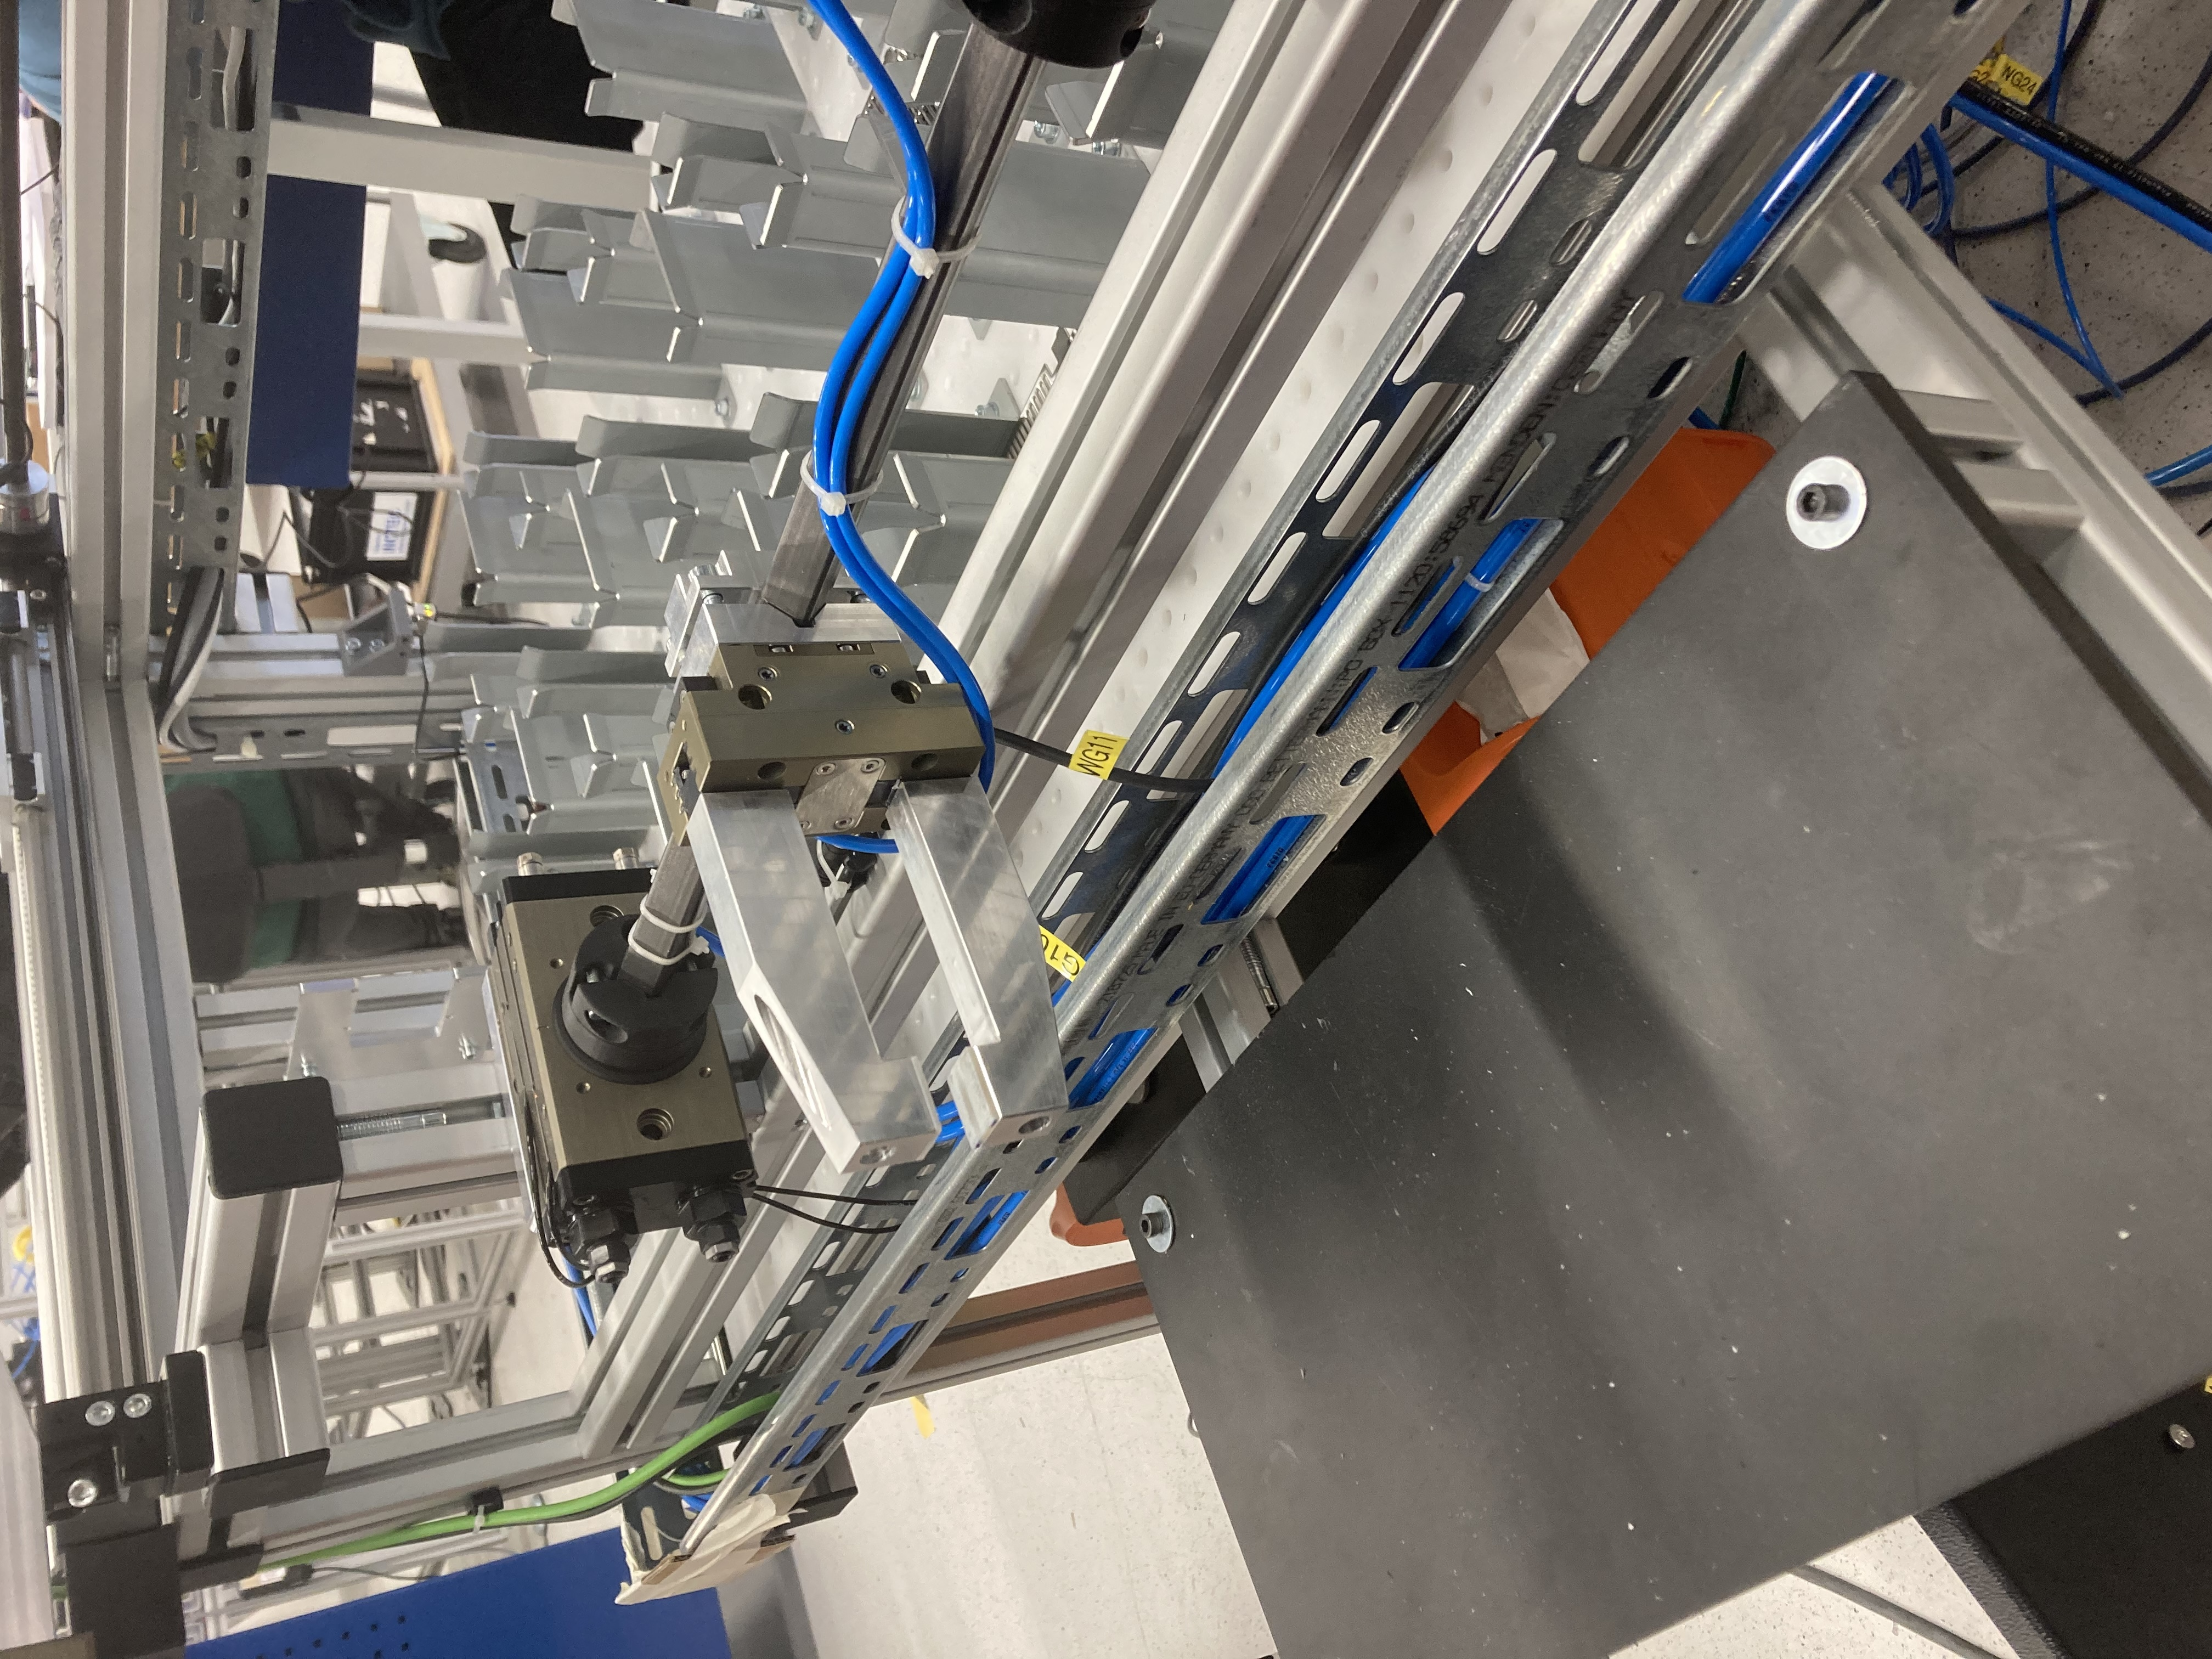
\includegraphics[width=\textwidth, angle=-90]{figures/unloading-station-gripper.jpg} % Replace with your image file
    %         \caption{}
    %         \label{fig:unloading-station-gripper}
    %     \end{subfigure}
    %     \caption{\parbox[t]{12cm}{Unloading station installations. a) Inspection Camera b) Pneumatic parallel gripper with pneumatic swivel unit}}
    %     \label{fig:unloading-station-installation}
    % \end{figure}
    
    \item As with the robot unit, different grippers (vacuum grippers, magnetic grippers, etc.) can be
    installed very quickly using a manual quick-change system, depending on the type of sheet metal part.
    \item After the gripper has unstacked a raw sheet, it is transferred to a pneumatic 180° swivel unit as shown in figure \ref{fig:unloading-station-gripper}, which in
    turn is equipped with a pneumatic parallel grippers. From
    there, the raw sheet is finally picked up by the robot unit described in the previous subsection \ref{subsec:robot-unit} after the
    exact position has been determined with the camera on the robot. In order to achieve reliable and
    precise positioning, a dark material is installed as background below the swivel unit. 
    \item As there is ample space between robot and unloading station, the inspection camera is installed directly on the unloading station as shown in figure \ref{fig:inspection-camera}.
    The robot comes in front of inspection camera after each bending to get the bending angle.
    \item All electronic
    components such as fuses, power supply units, etc. of the entire mobile robot unit, \textit{i.e.} not just those of
    the unloading station, are installed in several control cabinets below the gantry. This allows the
    unloading station to be used more flexibly later on different sheet metal bending machines. The same is
    planned for the pneumatic components such as switching valves, pressure regulators, pressure
    gauges, etc. Due to the flexibility and the space still available, the KR controller will also be
    placed in the back-side of this station.
    \item The front panel of unloading station has an HMI, an emergency stop button and the robot's teach pendant. Since the robot auto-starts the program
    when the power is turned on, the teach pendant is not used during operation. However, it is placed there for debugging or testing a new robot program.

    % \begin{figure}[h]
    %     \centering
    %     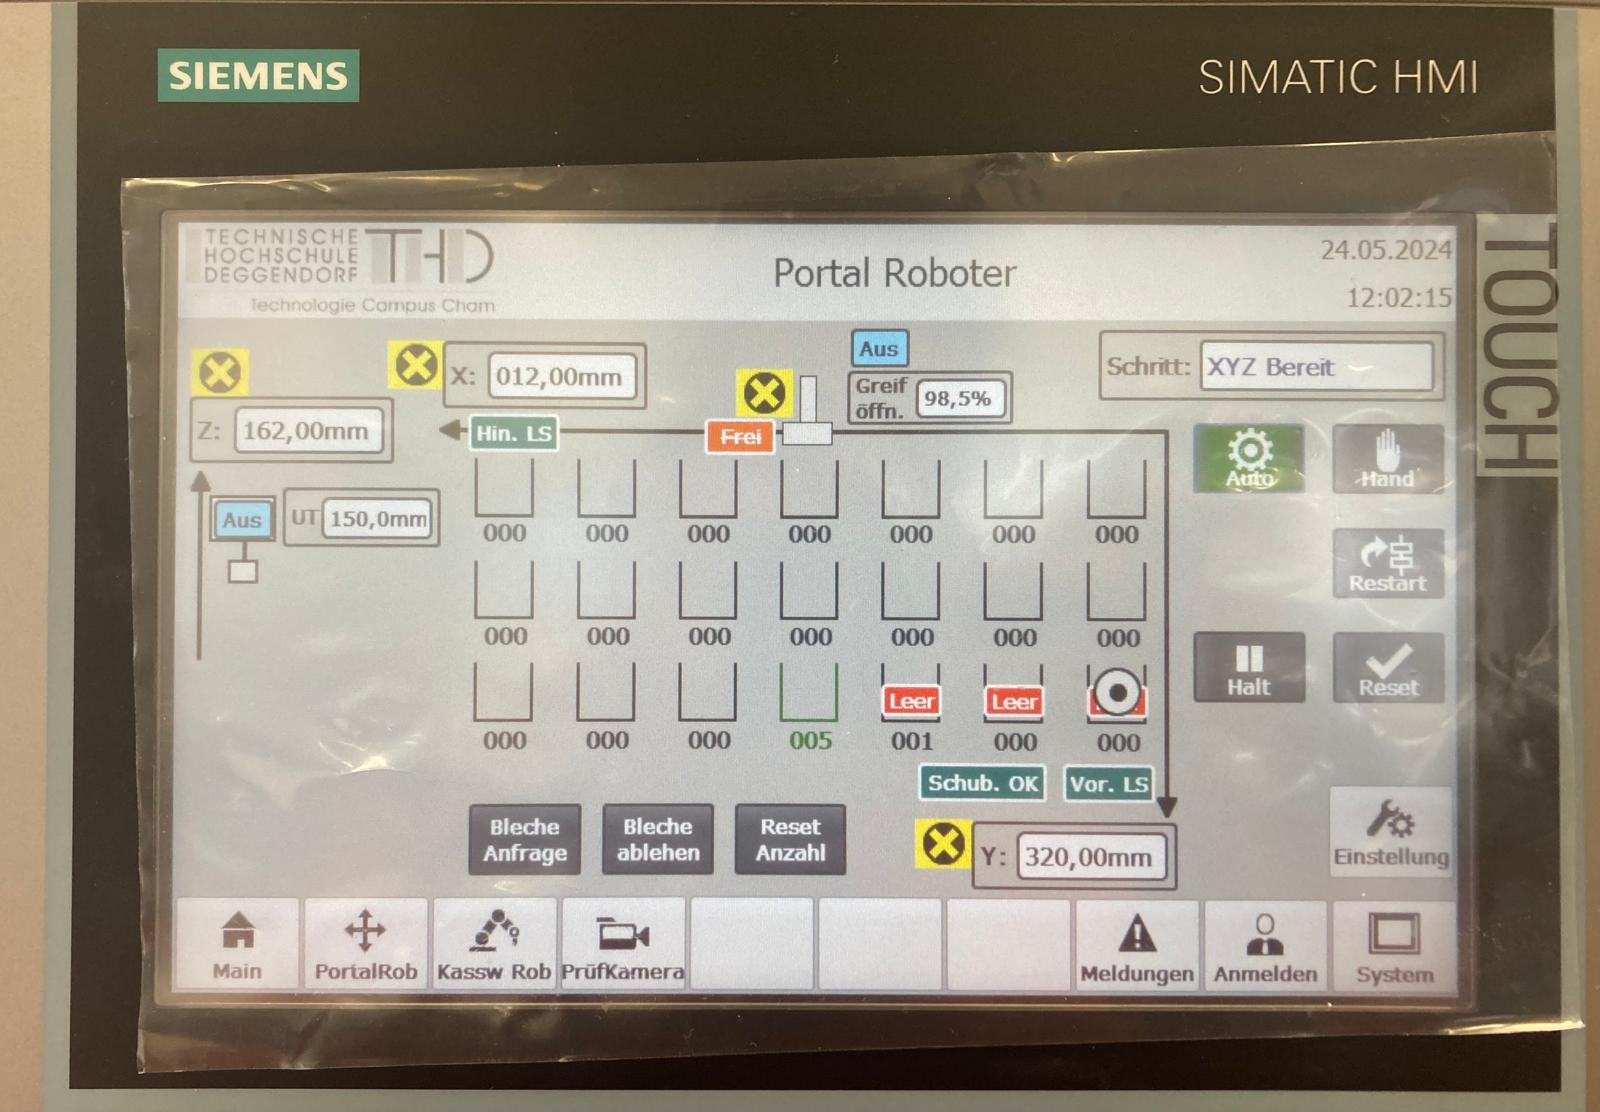
\includegraphics[width=0.6\textwidth]{figures/simatic-hmi.jpeg}
    %     \caption{HMI showing the sheet available in the unloading station}
    %     \label{fig:simatic-hmi}
    % \end{figure}

    \item An HMI control unit from Siemens is installed for the operation (start, pause, stop, etc.) of the entire robotic workcell and as
    a source of information about relevant process values, such as the number of sheets processed or failed in the current batch as shown in figure \ref{fig:simatic-hmi} The protective fence is attached with the unloading station, but contains a recess so that the HMI can be used at all times.
\end{enumerate}
